%Here you can see how to include an image in your document.
%
%\begin{sidewaysfigure}
%\centering
%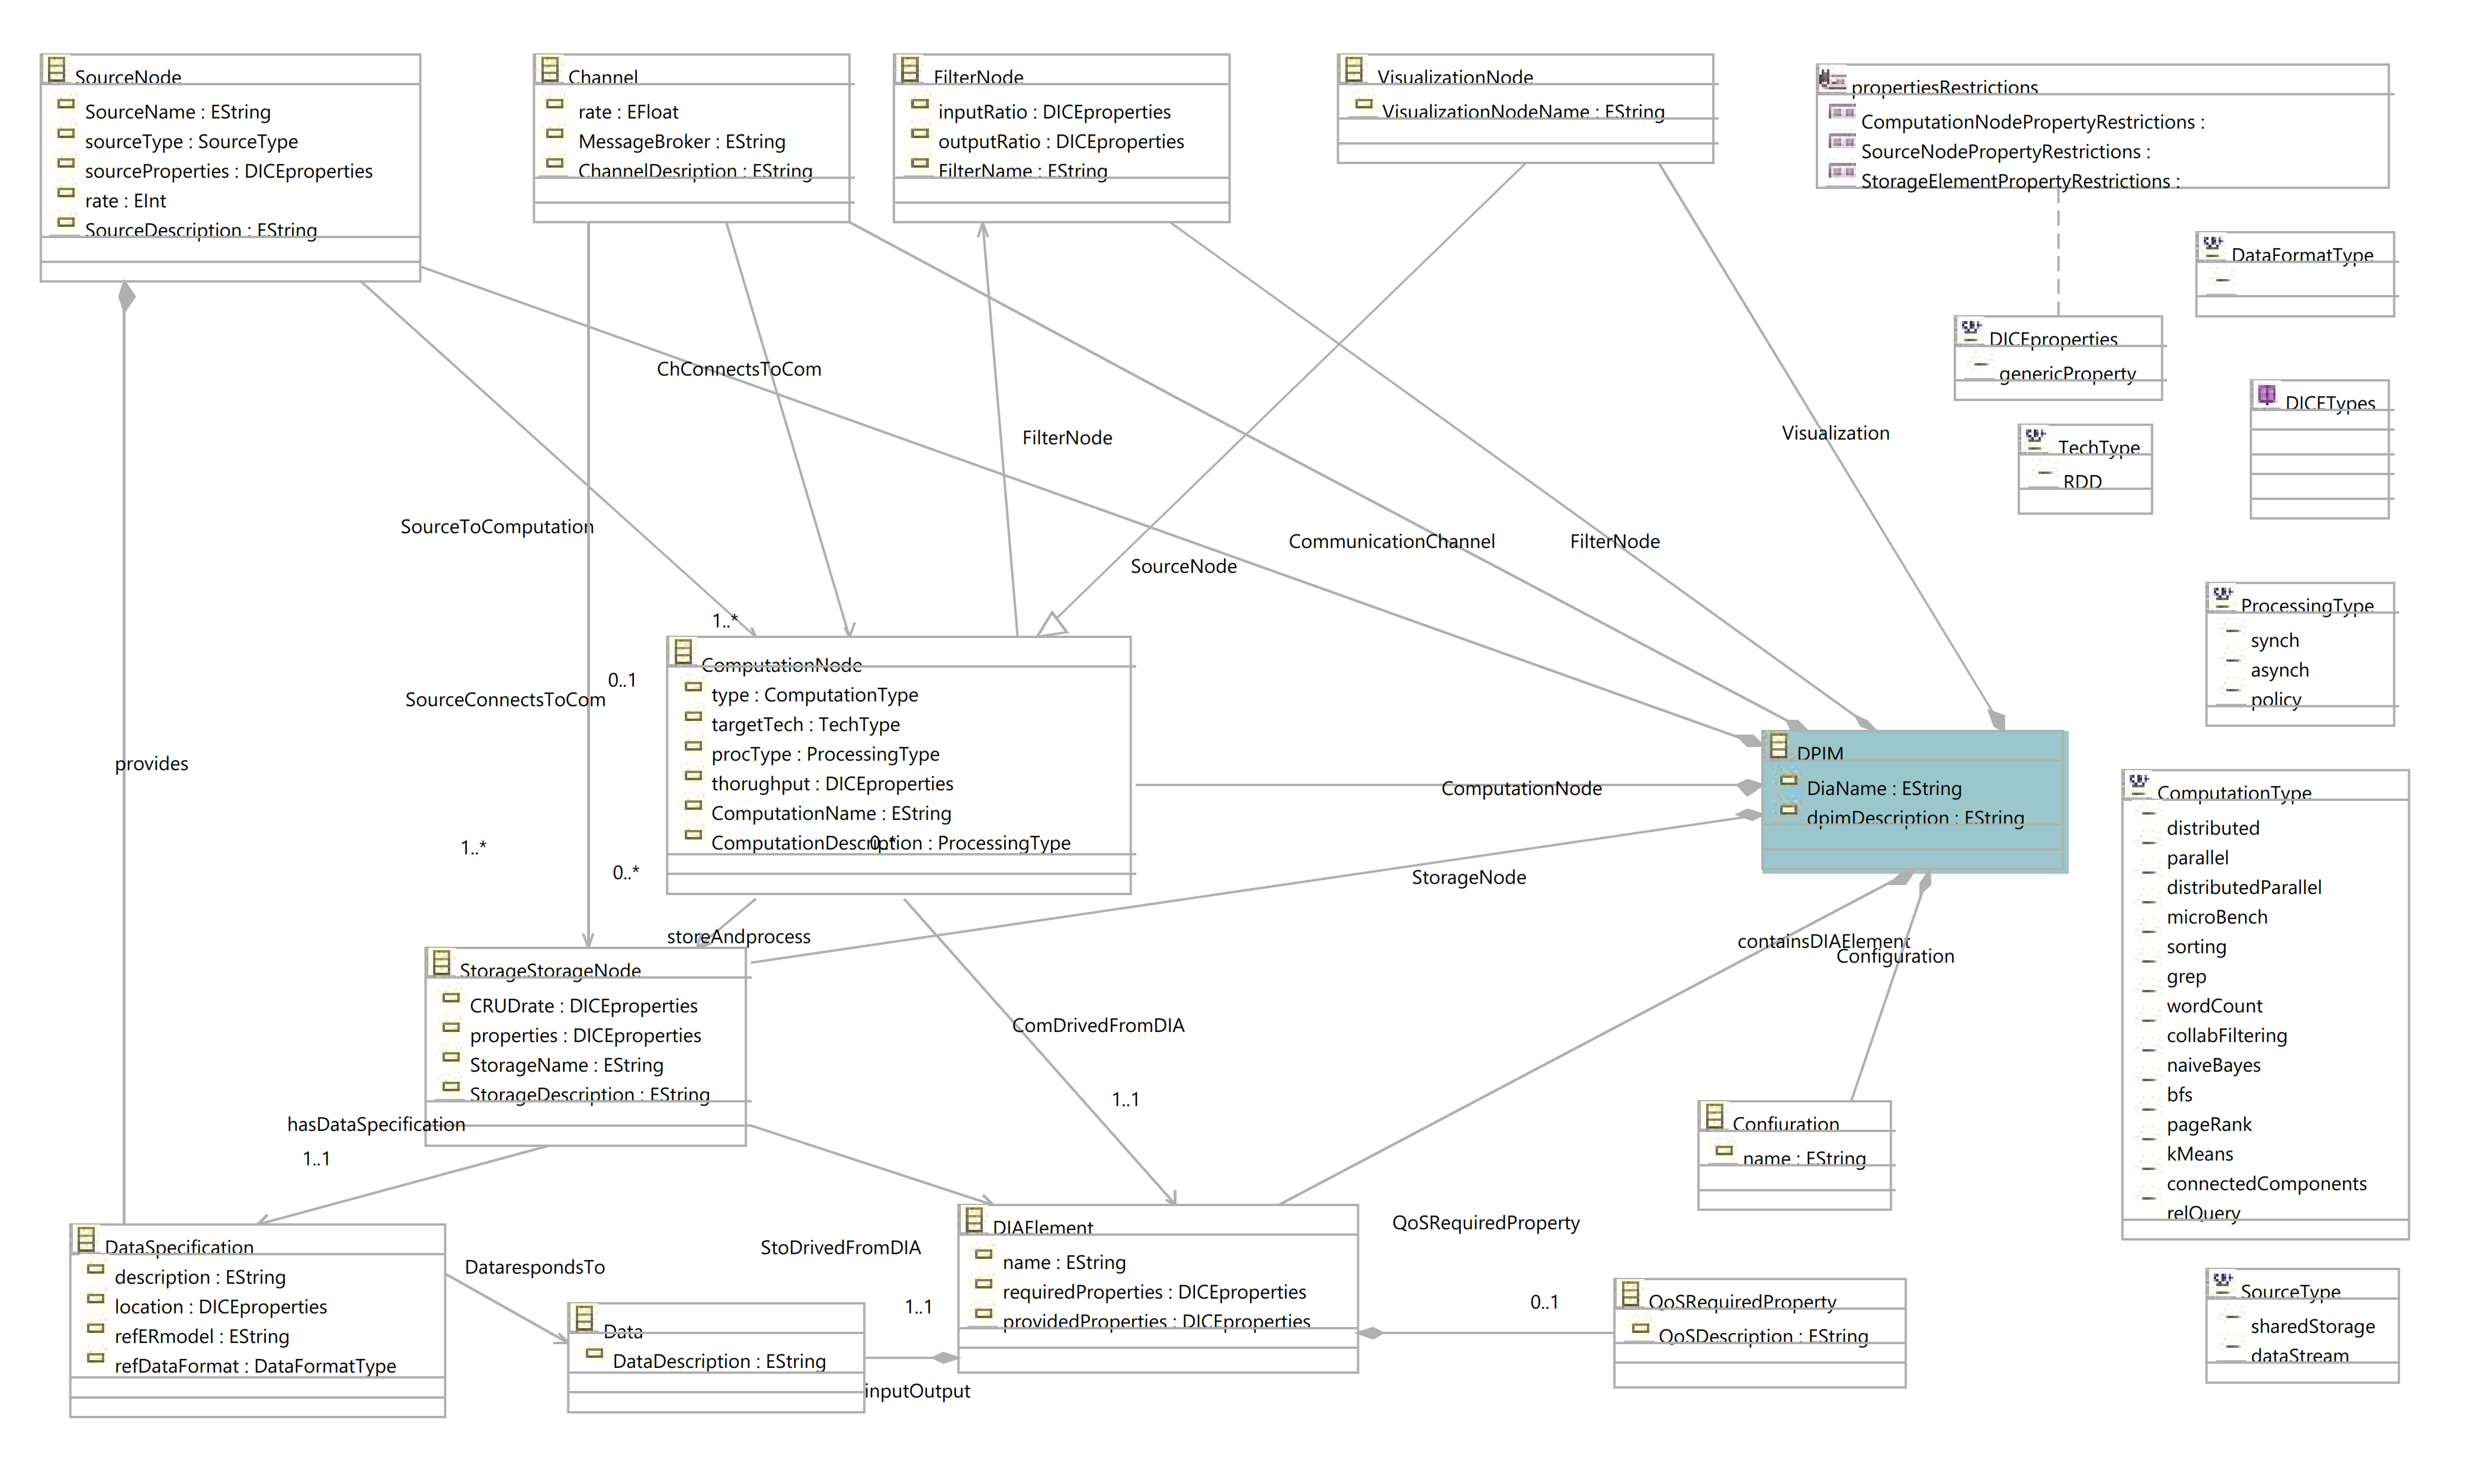
\includegraphics[width=\textwidth]{Images/11.png}
%\caption{\label{fig:metamodel}DICE DPIM metamodel.}
%\end{sidewaysfigure}

%\begin{figure}
%\centering
%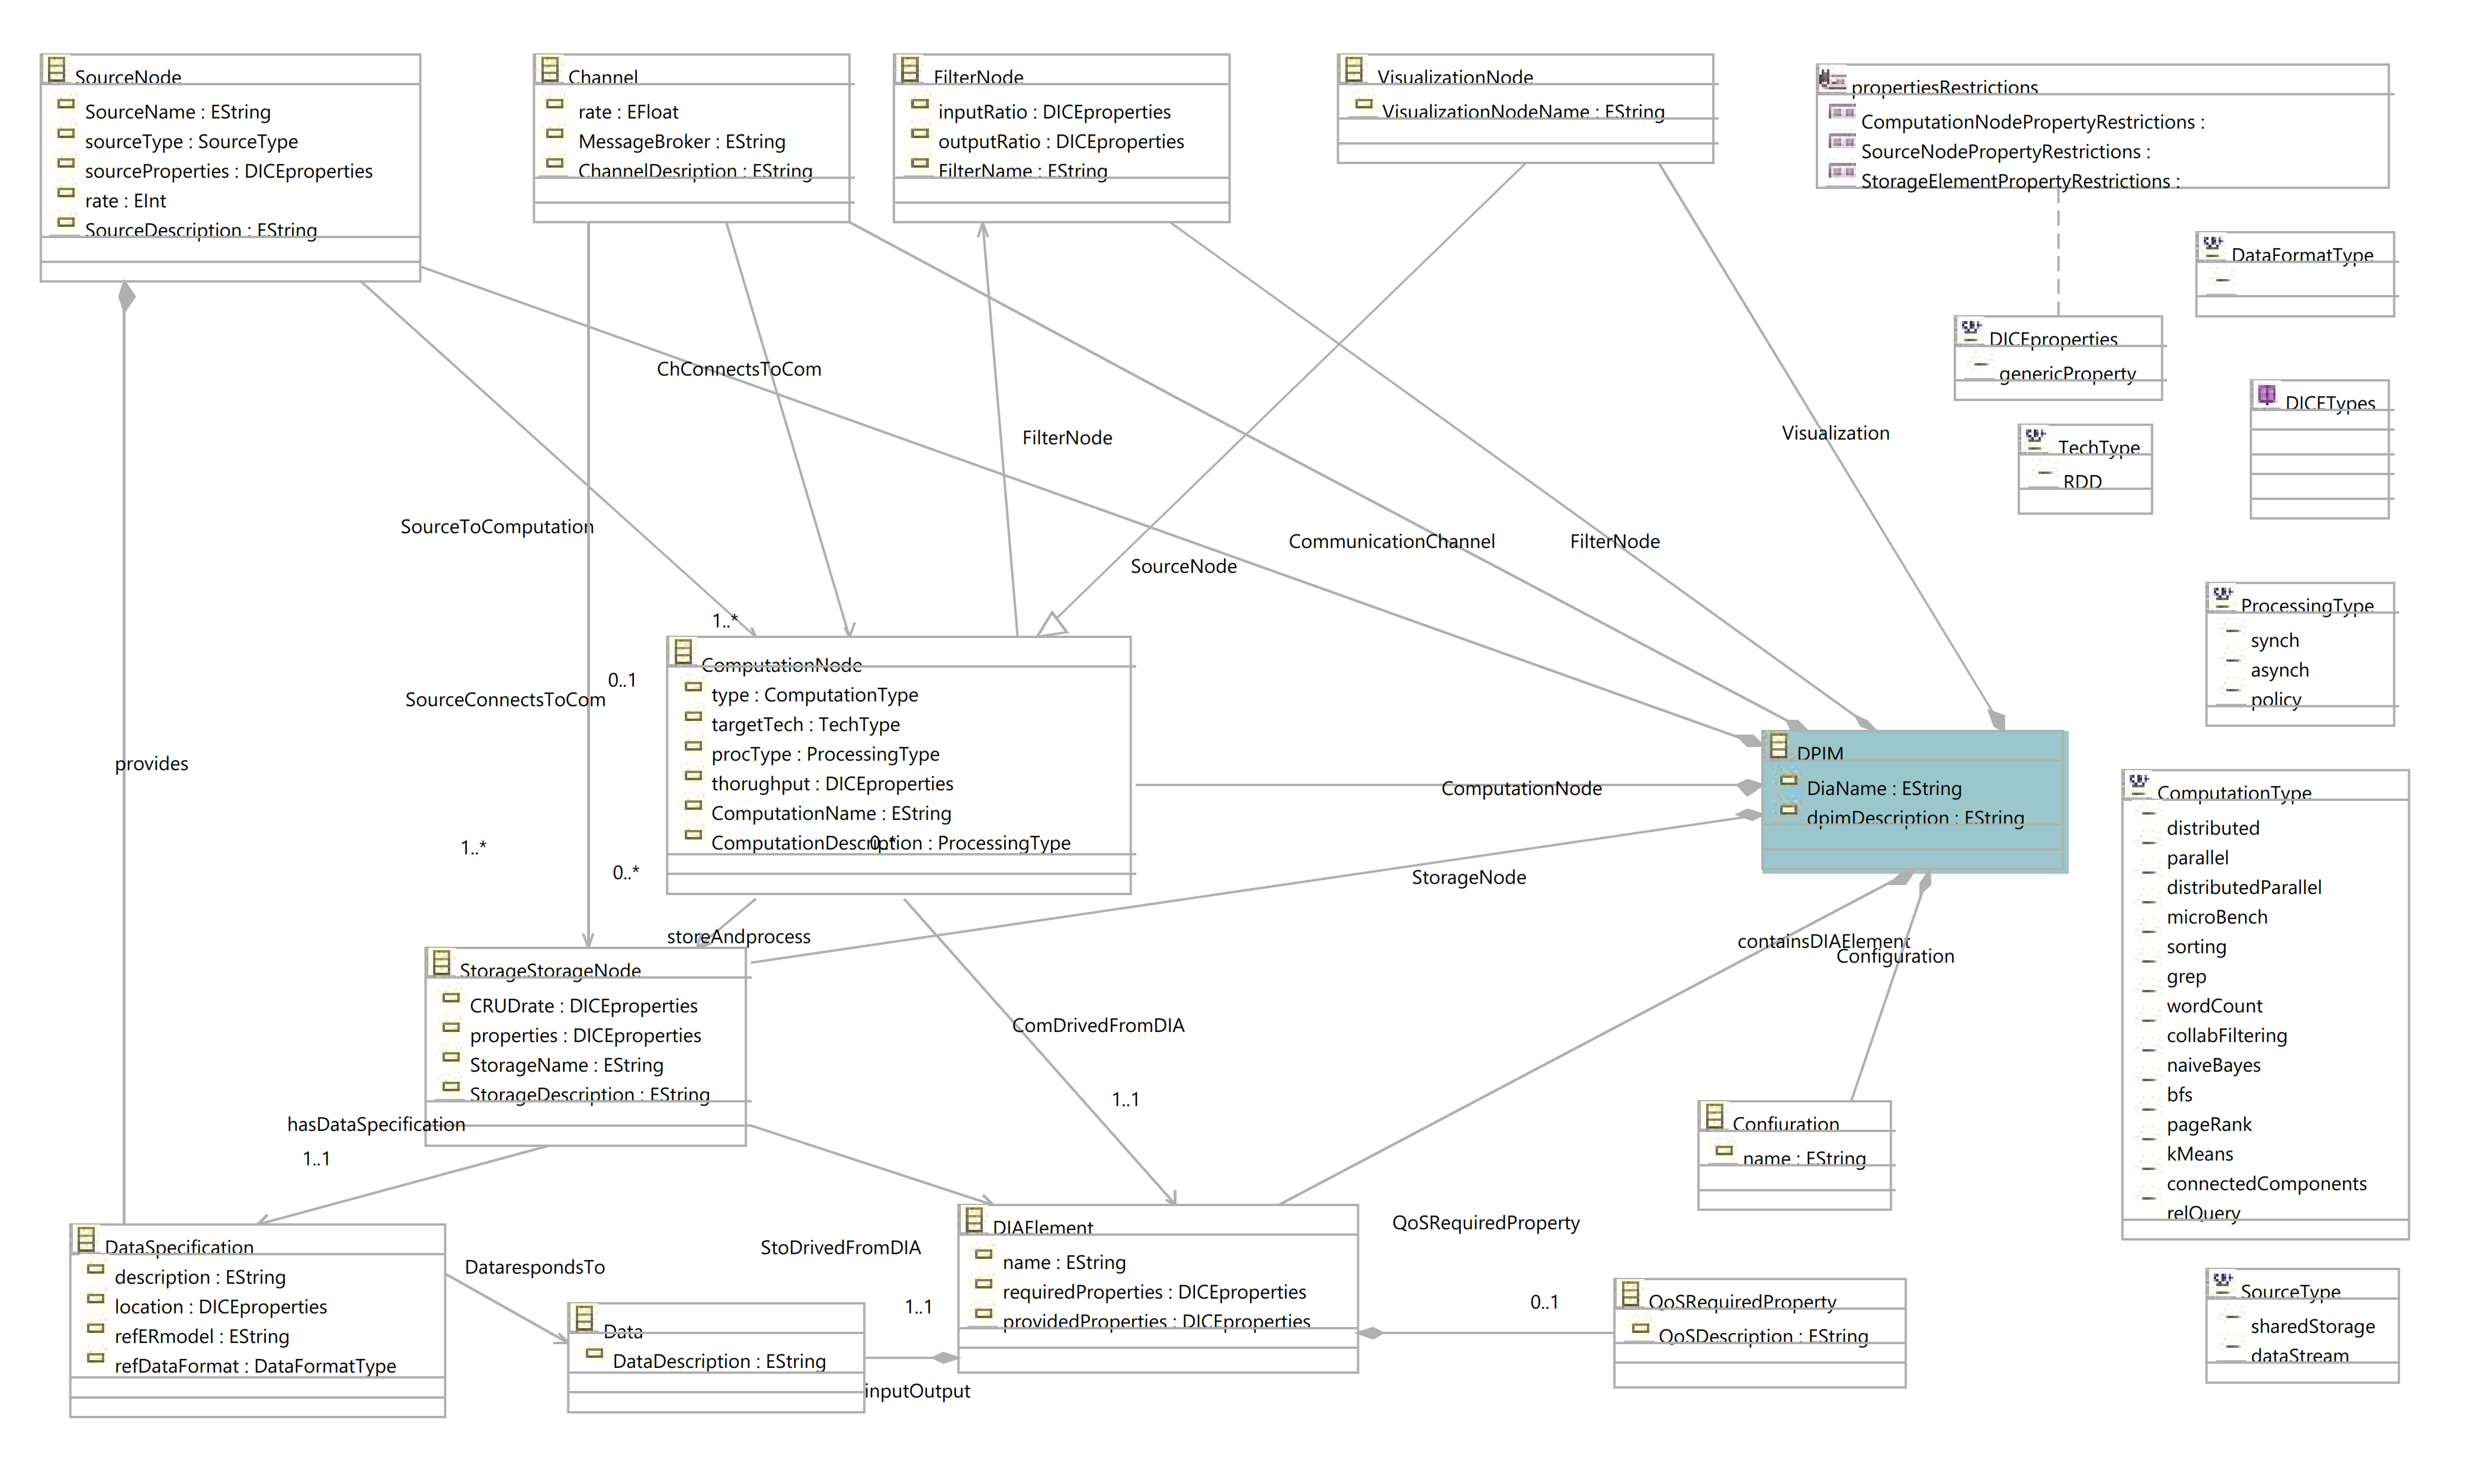
\includegraphics[width=\textwidth]{Images/11.png}
%\caption{\label{fig:metamodel2}DICE DPIM metamodel in portrait form.}
%\end{figure}

%Here is the command to refer to another element (section, figure, table, ...) in the document: \emph{As %discussed in Section~\ref{sect:overview} and as shown in Figure~\ref{fig:metamodel}, ...}. Here is how to %introduce a bibliographic citation~\cite{DAM}. Bibliographic references should be included in a \texttt{.bib} file. 

%Table generation is a bit complicated in Latex. You will soon become proficient, but to start you can %rely on tools or external services. See for instance this \href{https://www.tablesgenerator.com}{https://%www.tablesgenerator.com}. 

% -----------------------------------------------------
\subsection{Product perspective}

    \subsubsection{Scenarios} 
    
        \begin{enumerate}
            
            % - 1 -
            \item \textbf{A student wants to start using the Students\&Companies website}:
            \\Bob is a university student that is looking for an internship to enhance his CV and he decides to exploit a website to facilitate the research, so he connects to S\&C. After entering to the platform for the first time he must register himself on the web application; therefore, he selects the option \textit{"Register as student"} and he fills out sign-up form beginning the registration process providing his email, his full name and creating a password. After sending the data through the appropriate button the registration is done. At this point Bob will be able to fill out all the information required to complete the account such as \textit{Basic Information}, \textit{Academic Information}, and \textit{Skills}. Bob must also include \textit{CV} and \textit{Languages Spoken}. Until Bob fills out all the required information he will not be able to use the platform.

            % - 2 -
            \item \textbf{A company wants to start using the Students\&Companies website}:
            \\Bridgenix is a company that is looking for interns for an internship that want to offer and it decides to exploit a website to facilitate the research, so it connects to S\&C. After entering to the platform for the first time it must register itself on the web application; therefore, it selects the option \textit{"Register as company"} and it fills out sign-up form beginning the registration process providing its company email, its name and creating a password. After sending the data through the appropriate button the registration is done. At this point Bridgenix will be able to navigate on the homepage and to access to its personal profile in which it can fill out all the information required to complete the account such as a short description of the company, the location and the logo.

            % - 3 - 
            \item \textbf{A university wants to start using the Students\&Companies website}:
            Mordor Institute of Technology is a university that would like to monitor the internships of its students, connects to S\&C. After entering to the platform for the first time it must register itself on the web application; therefore, it selects the option \textit{"Register as university"} and it fills out sign-up form beginning the registration process providing its university email, its name, its main address, its university mail, the link to the institutional website, and creating a password. After sending the data through the appropriate button the registration is done.
         
            % - 4 -
            \item \textbf{A student changes his personal information}:
            \\ Jack has finished some new projects, updated his CV and took a new certification. He logs into S\&C to update his personal information. There he can modify many fields and save the changes. 
            
            % - 5 -
            \item \textbf{A company changes his personal information}:
            \\ The company WeInnovate decides to update his profile on S\&C. On the profile page, it can make changes on the company information.  

            % - 6 -                 
            \item \textbf{A university changes his personal information}:
            \\ The Horizon University decides to update his profile on S\&C. On the profile page, it can make changes on the university information.
            
            \newpage
            % - 7 -
            \item \textbf{A company wants to post a new internship and review student applications}:
            \\After setting up its profile, Bridgenix can post available internships by navigating to the internship creation section. Here, the company can specify details in the \textit{Internship Role Description}, including the title, responsibilities, required skills, qualifications, and the application process.
            It can also provide \textit{Application Details}, to guide students on how to apply for the internship, specifying any required documents. Additionally, Bridgenix may list \textit{Perks and Benefits} associated with the position, such as compensation, additional benefits, and other perks to make the role more attractive to prospective interns. Once the company has fully set up the internship details, it can publish the opportunity on the platform. 
            Every time a student applies for the position, Bridgenix will receive a notification, allowing the company to review the application submitted. For each candidate, the enterprise can access complete details, and if is interested, initiate the selection process to begin evaluating the applicant.
            
            % - 8 -
            \item \textbf{A student proactively searches for an internship}:  
            \\Anita is a student registered to S\&C. Once she is logged into the platform, she can easily find the \textit{Available job search} button. By clicking it, the student will be redirected to another page of the website where she can type into the search bar specific keywords or she can apply specific filters on the search. After issuing the search, Anita will see a list of all the suitable internship positions with synthetic details about the company which is offering it. If she clicks one of them, she will be able to see more details on it.
            
            % - 9 -
            \item \textbf{A company looks for a match}   
            \\The company WorkInc is registered to the platform and has some open positions for internships. The person who is logged in for the company can click the button \textit{"Match Internship"} on the page of a specific internship, then the platform runs analytics to match it with as many students as possible. Internship pages feature a section \textit{"Matching Candidates"} where there is a list of all the suitable candidates for the positions. 

            % - 10 -
            \item \textbf{Universities monitor the internships of their students }
            \\ The university of Erewhon has a list of all the students enrolled to it that are doing an internship. The university can further look into the internship and getting to know the details of it (the company, the duration, location, role title, etc.). However, the university can look the status of an internship only once it is started, not before.
            
            % - 11 -
            \item \textbf{Users interact in the application process}
            \\ The company JobCo has to evaluate some selected students who applied to one of his internships. JobCo will schedule an interview providing the meeting link along with the specified date and time. Based on the interview performance, JobCo will extend an offer to the best students, wait-list some others and reject all the other. The students can accept or refuse the final offer made by the company or acknowledge the fact that they were wait-listed or rejected.
            
            % - 12 -
            \item \textbf{Users keep track of the internship }
            \\ The company JobCo can leave private notes to the student, including suggestions, criticisms but also news about the internship. On the other hand, Tony, the student who is carrying out the internship, can communicate problems. Both JobCo and Tony can see the status of the internship and read information regarding the internship, that either one of the two has written on the platform.
            
            % - 13 - 
            \item \textbf{Universities monitor the internships of their students }
            \\ The university of Erewhon has a list of all the students enrolled to it that are doing an internship. The university can further look into the internship and getting to know the details of it (the company, the duration, location, role title, etc.). However, the university can look the status of an internship only once it is started, not before.
        \end{enumerate}
        
        \newcommand{\mycomment}[1]{}
        \mycomment{
            \begin{enumerate}[label=\textbf{[\arabic*]}, left = 0 pt, align = left]
            % ----
            \item \textbf{Student Application to Internship}                      
            \\Once a student finds an internship that might interest them, they can click on the preview of the placement, which will redirect to the company's private webpage. By pressing the \textit{"Apply Now"} button, a form will appear where the student must enter all the required information specified by the company. Once all the fields are completed, they can submit their application by clicking the \textit{"Submit"} button.
            
            % ----
            \item \textbf{Company Review of Student Applications}           % DONE 
            \\Once a company has posted one or more internship proposals, it will be able to see the applications submitted for each proposal by clicking on \textit{"Sent applications"}, which will redirect to a dedicated webpage displaying all the applications for a particular internship. For each application, brief information is shown on the screen, and the company can access the complete details by clicking the \textit{"More details"} button. If the company is interested to the student, it can click on \textit{"Start Selection Process"} to begin evaluating the candidate and will be prompted a calendar to indicate the available days and time slots.           
            
            \item \textbf{Feedback Submission by Student Post-Internship}        
            \\
            \item \textbf{Feedback Submission by Company Post-Internship}        
            \\
            \item \textbf{Internal Status Update by Student}                     
            \\
            \item \textbf{Internship Status Update by Company}                   
            \\
            \item \textbf{Notification of New Internship Opportunities}          
            \\
            
            \end{enumerate}
        }
    
    % -----------------------------------------------------.
    \newpage
    \subsubsection{Domain Class Diagram}
    To capture the different classes, their methods and their interactions we drew the following domain class diagram
        \begin{figure}[h!]
            \centering
            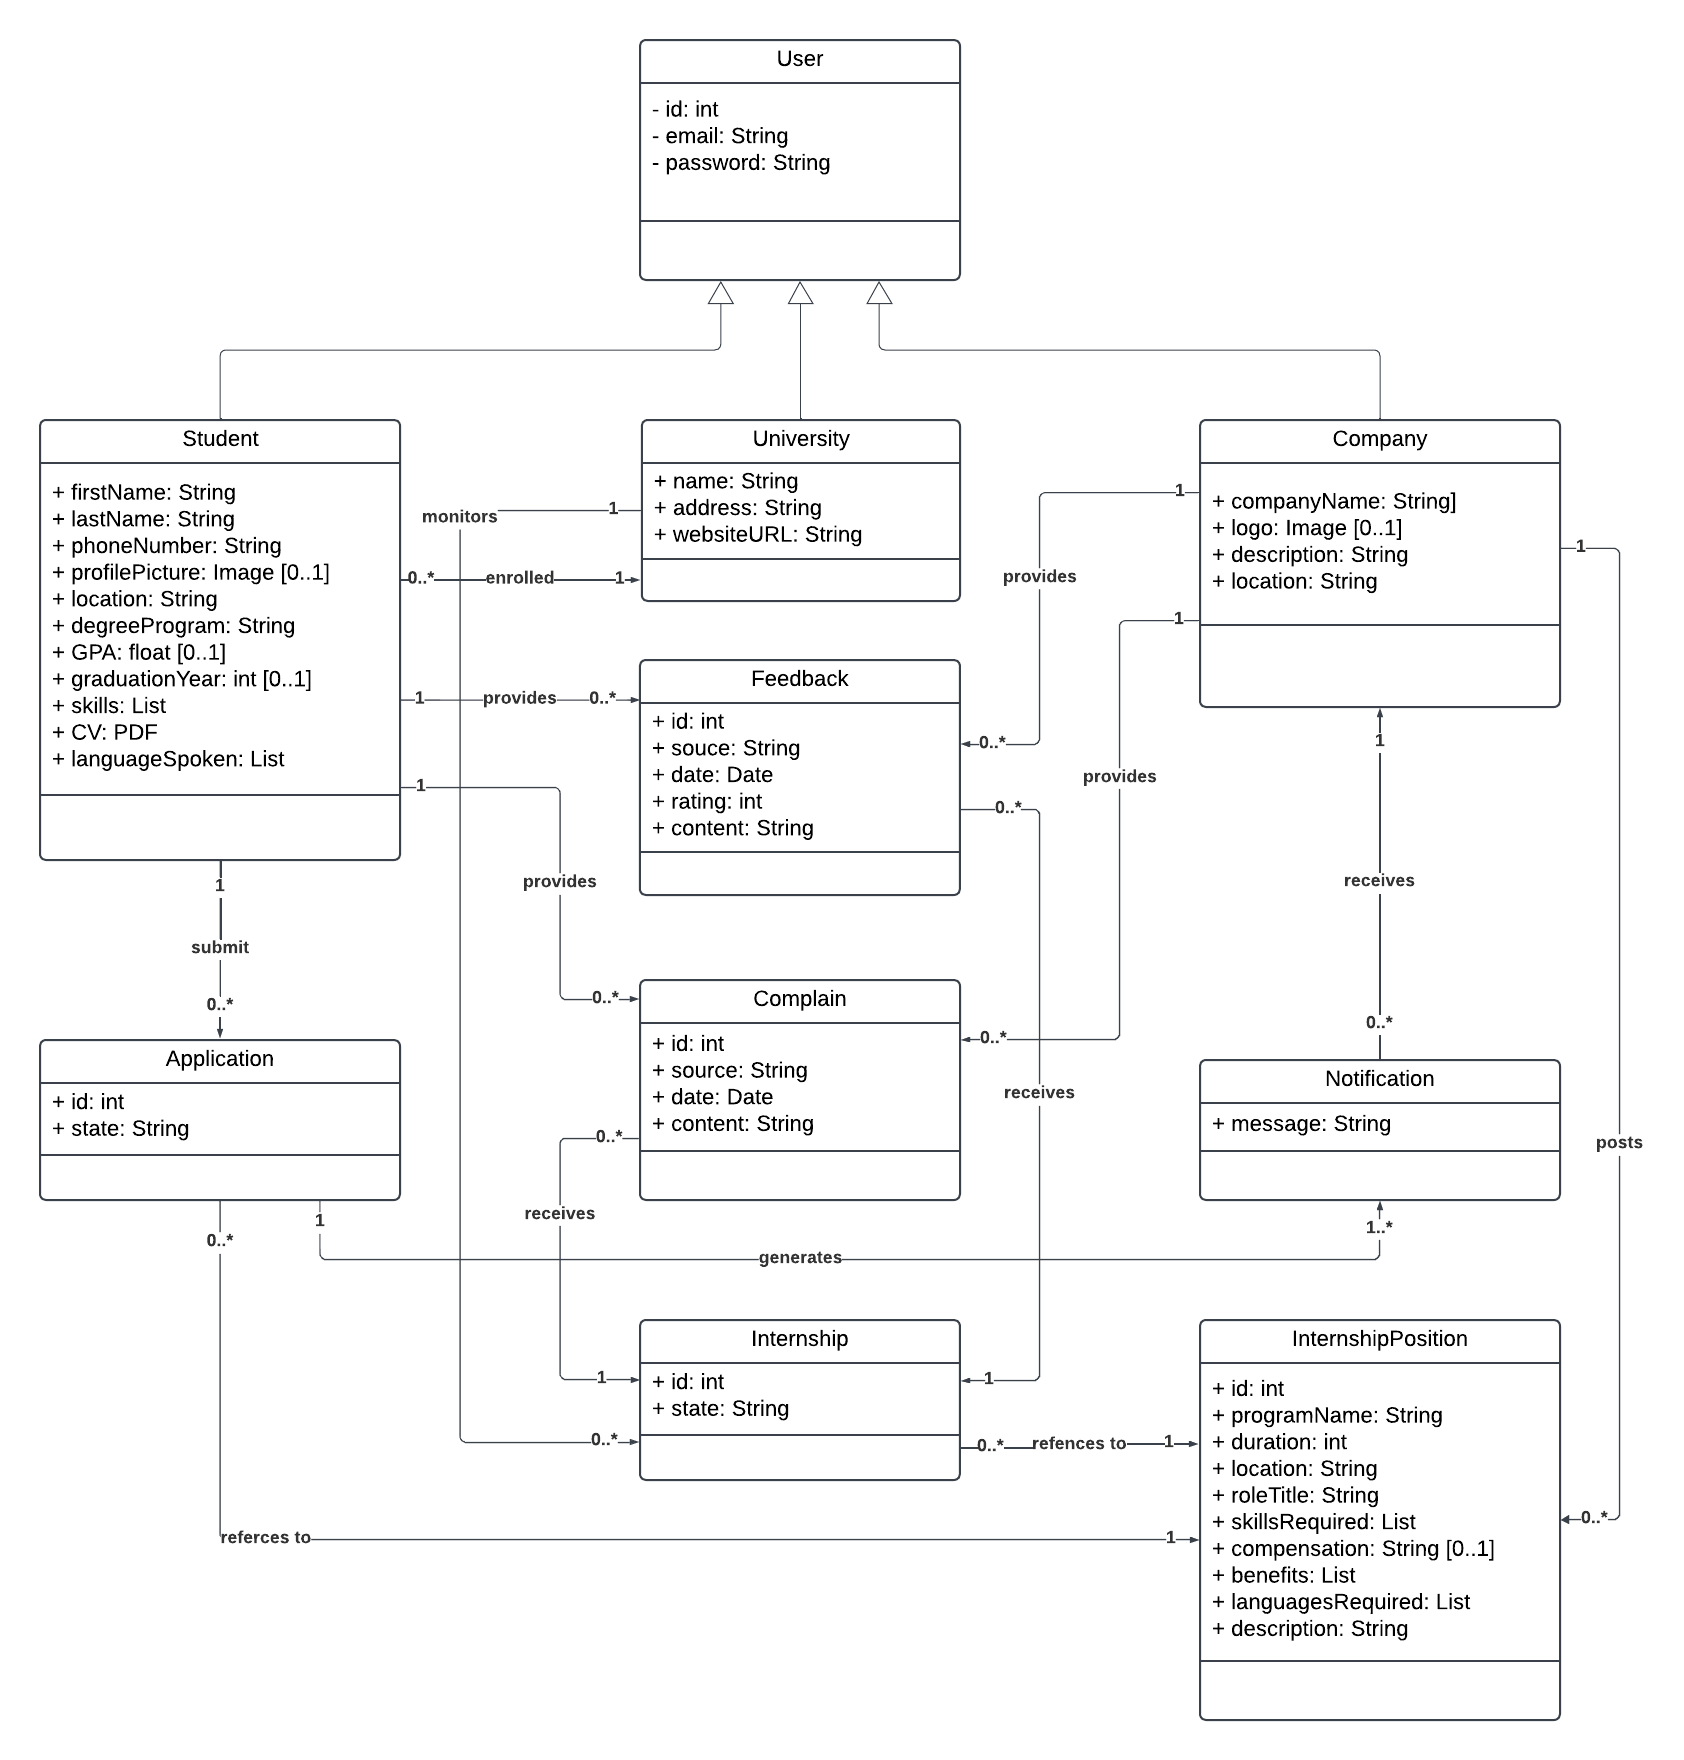
\includegraphics[width=1\textwidth]{RASD/RASDdiagrams/2.1.2_DomainClassDiagram.png}
            \caption{Class Diagram}
            \label{fig:example}
        \end{figure}
    
    
    % -----------------------------------------------------
    \newpage
    \subsubsection{State Diagrams}
        The most crucial aspect of the application is the creation and evolution of the internship positions on the platform. Not to leave any room for doubts, we explain both the point of view of the company and the one of the student.
        \\
        A company can close an internship position whenever it wants to. Once it closes the internship, the applications who were accepted but not confirmed or not refused, the pending applications, and the applications needing an further assessments are automatically rejected. Instead, for those who confirmed, we consider the moment of the closing of the open position by the company as the moment in which they start their internship.
        \\
        \begin{enumerate}[label=\textbullet, itemsep=0em]
            \item \textbf {Company's Perspective}
            \\The following is the point of view of the company:
            \begin{figure}[h!]
                \centering
                
\includegraphics[width=1\textwidth]{RASD/Images/CompanyPOV.png}
                \caption{The evolution of an internship position on the platform from the point of view of a company}
                \label{fig:example}
            \end{figure}
            \\
        
            \item \textbf {Student's Perspective}
            \\The following one, instead, is the point of view of a student:
            \begin{figure}[h!]
                \centering
                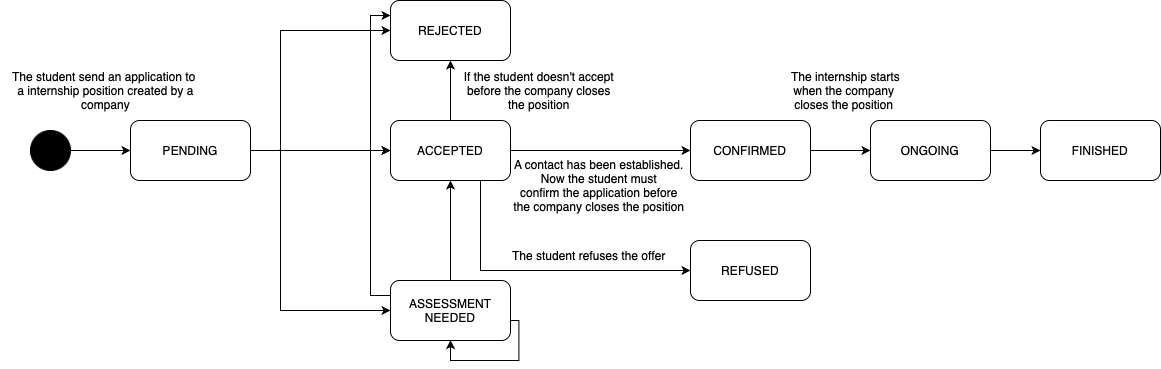
\includegraphics[width=1\textwidth]{RASD/Images/StudentPOV.png}
                \caption{The evolution of an internship position on the platform from the point of view of a student}
                \label{fig:example}
            \end{figure}

        \end{enumerate}
        
% -----------------------------------------------------

\subsection{Product Functions}
    \begin{enumerate}
        % - 1 -
        \item \textbf {Sign Up and Log In}             
        \\ The users sign up to the platform by providing an email and a password. A registered user logs in to the platform by providing the same information. At the moment of sign up it is necessary to indicate whether the account is related to a company, to a university or to a student, since the three types of account are treated differently inside the platform.
        
        % - 2 -
        \newpage
        \item \textbf {Profile Information Filling}   
        \\ The users fill his profile information. Companies will be asked for its name, the headquarters location,  a brief description of their business activities and it can also include the company's logo. Universities will be asked for the name, main address, institutional mail and URL of the official website. Students will be asked for name, surname, phone number, education, skills, languages spoken and CV. A part of the information is published on the platform, another part of the information is used by the recommendation system.
        
        % - 3 -
        \item \textbf {Internship Position Creation}
        \\ Companies can create new internships positions by establishing the duration, the work place, the role title, the responsibilities, the required experience, the required skills, languages required, and the salary range and benefits.

        % - 4 -
        \item \textbf{Internship Search}
        \\ Students can search for internship opportunities using various filters based on their preferences, such as location, role, required skills, and salary range. Once the filters are applied, the platform presents a list of relevant internship positions. Students can browse the list and click on each position to view detailed information.

        % - 5 - 
        \item \textbf{Internship Application}
        \\ After reviewing the available internship positions, students can apply to one or more internships that align with their interests. By clicking the "Apply" button, the student sends an application to the company, expressing their interest in the position. The company will then review the application as part of their selection process.
        
        % - 6 -
        \item \textbf {Management of the Selection Process}
        \\ Companies see the profiles of students who applied to an internship. S\&C enable them to configure the selection process based on their needs. They can reject students who applied to an internship position after checking their qualifications on their profiles; they can directly accept one or more of them. Companies can propose interviews to assess the preparation of students who applied for an internship position and finalize the decisions after the tests or requesting an online interview.

        % - 7 -
        \item \textbf{Situation Monitoring by University}
        \\ Universities can monitor the status of internships their students are participating in. They can track the progress of the internship, review feedback provided by companies, and assess whether the students' educational goals are being met. This monitoring function allows universities to stay informed about their students' experiences and intervene if necessary, without being able to directly modify or communicate within the internship process.
        
        % - 8 - 
        \item \textbf {Communication Space}
        \\ After an internship is started, both the students and companies have dedicated sections of the website to exchange information, communicate problems, indicate suggestions, make announcements (all regarding the internship) such that both of the interested parties can benefit from the sharing of information. 

        % - 9 - 
        \item \textbf {Feedback Management}
        \\ After the internship is finished the platform asks both the company and the student to rate and review each other. Moreover it asks both parties for suggestions. Collecting this kind of information is particularly important to feed and improve the recommendation system.
        \\
    \end{enumerate}

% -----------------------------------------------------
\subsection{User Characteristics}
    Users of S\&C are divided into three distinct categories, each with specific roles and responsibilities that reflect their interaction with the internship process:
    
    % - 1 -
    \subsubsection{Students}
    Students are the main beneficiaries of the S\&C platform, using it to find internship opportunities and develop their professional skills. Their responsibilities and capacities include:
    \begin{enumerate}[label=\textbullet, itemsep=0em]
        \item \textbf{Internship Search}
        \\ Students can search through the available internships by applying various filters such as location, role, required skills, and salary range to find positions that match their career goals.
        
        \item \textbf{Application for Internship Positions}
        \\ Students can apply for internships directly through the platform.

        \item \textbf{Participation in the Selection Process}
        \\ Once a student has applied, it may be necessary to go through a selection process set up by the company offering the internship. This could include interviews to determine their suitability for the position.

        \item \textbf{Accepting or Rejecting Offers}
        \\ Once a company makes an internship offer, students can review the details and choose to accept or reject the offer. This ensures that students have control over their internship decisions.

        \item \textbf{Communicating with the Company}
        \\ During the internship, students can use the platform to communicate directly with the company, facilitating the exchange of information, addressing requests or providing updates on their progress.
        
        \item \textbf{Providing Feedback}
        \\ After completing an internship, students can provide feedback on their experience, helping future applicants and companies to assess the quality of internships. This feedback can be used to improve the platform and the internship experience itself.
    \end{enumerate}
    
    % - 2 -
    \subsubsection{Companies}
    Companies use the platform to find talented students for internship opportunities and to manage the selection and monitoring process. Their main features include:
    \begin{enumerate}[label=\textbullet, itemsep=0em]
        \item \textbf{Creating Internship Openings}
        \\ Companies can create and publish internship opportunities on the platform. They provide details such as the role, skills required and other relevant information to attract suitable candidates.

        \item \textbf{Definition of the selection process}
        \\ Companies are responsible for defining the stages of selection of trainees. This includes the definition of interview schedules and the determination of assessment criteria to ensure that the best candidates are selected for the role.

        \item  \textbf{Tracking Internship Progress}
        \\ During the internship, companies can monitor the status of internship stages, providing continuous mentoring and addressing any problems that arise.

        \item \textbf{Provide feedback on students}
        \\ After completion of the internship, companies are able to provide feedback on student performance which can influence future internship opportunities or job offers for the student.
    \end{enumerate}
    
    % - 3 -
    \subsubsection{Universities}
    Universities have a limited role within the S\&C platform, focusing exclusively on monitoring the internships undertaken by their students. Their functionality includes:
    \begin{enumerate}[label=\textbullet, itemsep=0em]
        \item \textbf{Monitoring Student Internships}
        \\ Universities can track the internships their students are participating in through the platform. This allows them to stay informed about the progress and status of these experiences without directly intervening or influencing the process.
    \end{enumerate}
    
% ------------------------------------------------------
\subsection{Assumptions, Dependencies and Constraints}
    % ---
    \subsubsection{Regulatory Policies}
        Personal information will be processed in compliance with GDPR rules.
    
    % ---
    \subsubsection{Domain Assumptions}
    \begin{enumerate}[label={[D\arabic*]}]
        \item {Students insert correct information about their skills and experience}
        \item {Students apply to jobs in countries where they have a work permit}
        \item {Students provide valuable feedback when asked for it}
        \item {Companies offer existing and legal contracts for the internships}
        \item {Companies insert correct information about the internships}
        \item {Companies periodically review information about the internship candidates}
        \item {Companies provide valuable feedback when asked for it}
        % \item {Most of universities are contacted before the website is online so that most of them are already present on the platform, when the website is deployed}
        \item {Students raise problems through the platform}
        \item {Companies use the platform as principal mean of communication regarding the internships }
        \item {Universities must register on the platform before their students can create accounts, as students are required to link their profiles to their university}
    \end{enumerate}